\documentclass[11pt, letterpaper]{article}
\usepackage{graphicx}
\title{Lab T report}
\begin{document}
\maketitle
\section{Administrative}

Team names: Graham Benevelli Jake Wilke\\
Team uteids: grambo jlw3599\\
Slip days previously used: 0\\
Slip days used this project: 0\\
Slip days remaining:?\\

\section{Part 1: Basic synchronization}

{\em At most 1/2 page -- Discuss high level design, any issues/known
  bugs}

\subsection{Evaluation}

\centerline{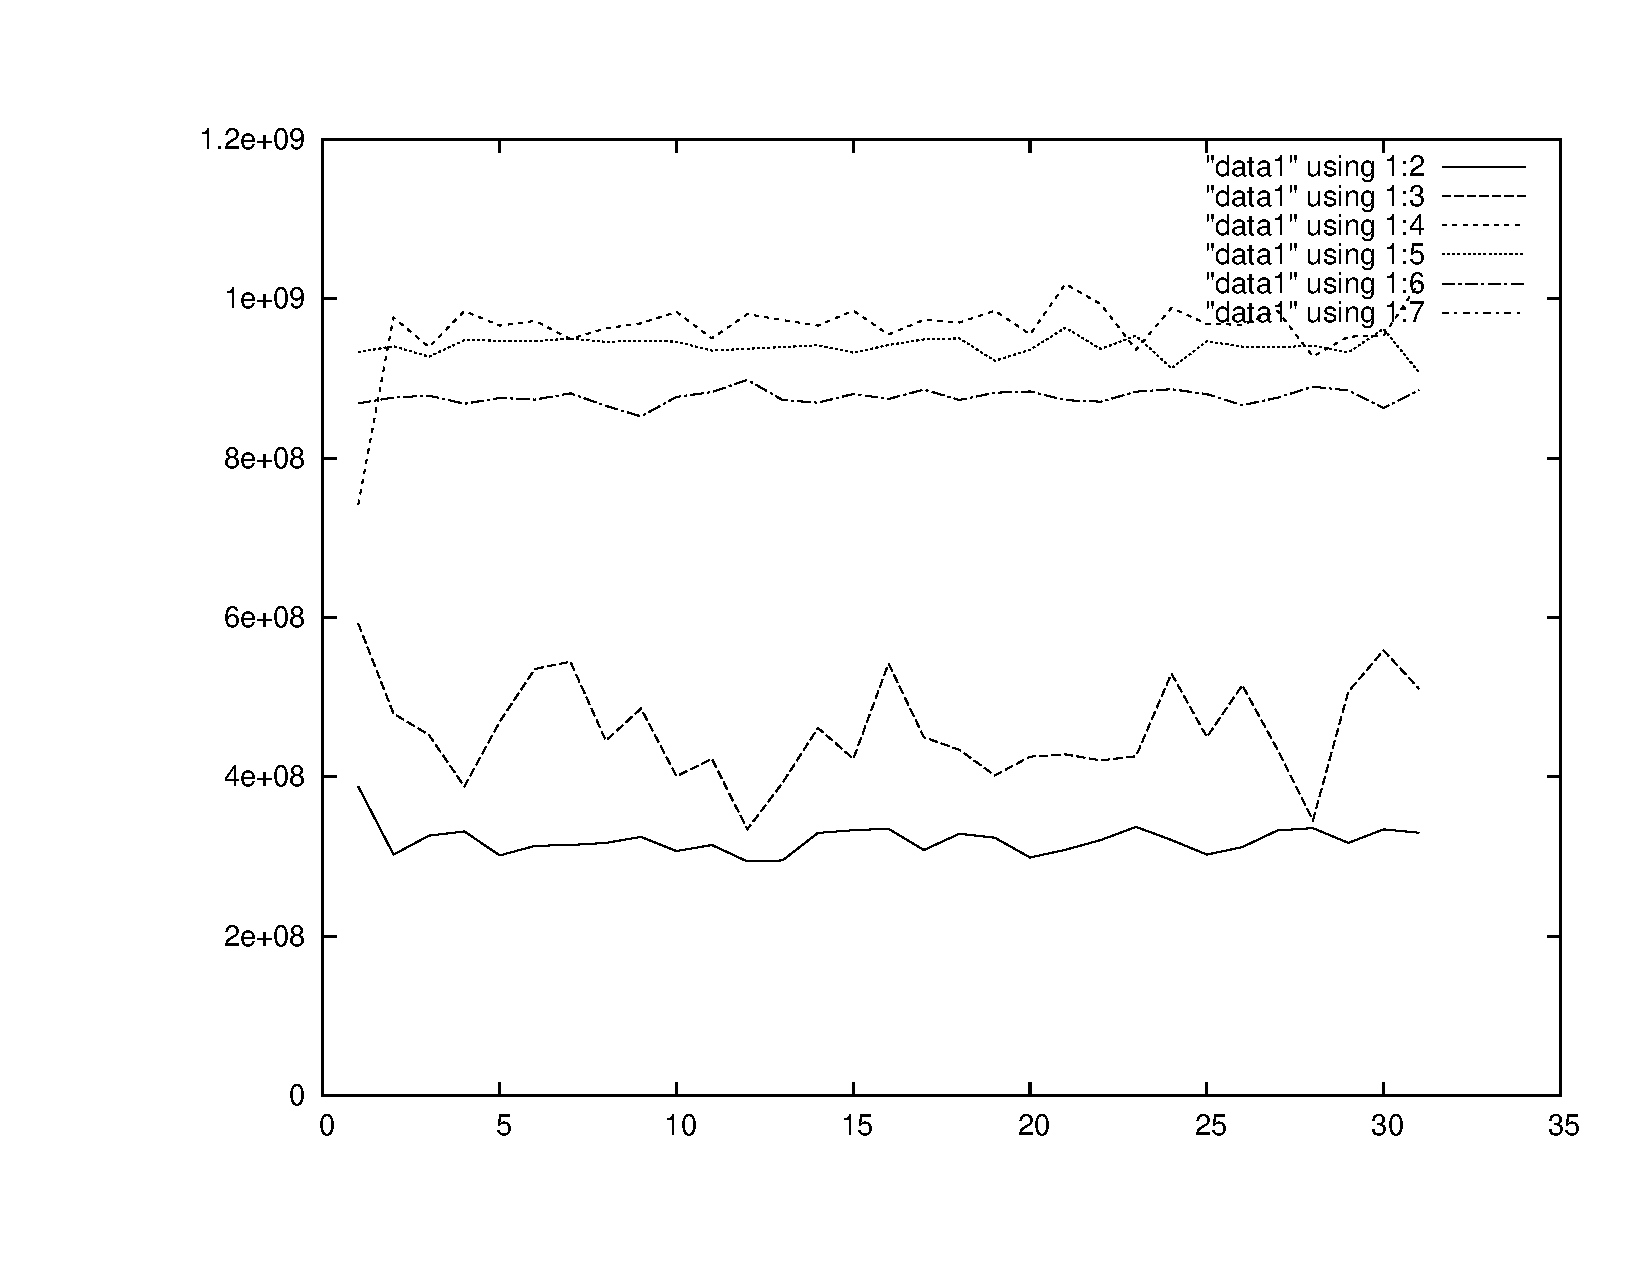
\includegraphics[width=3in]{plot1}}

{\em Explain graph; identify/explain any
  interesting/unexpected/important features}


\centerline{
\includegraphics[width=3in]{plot1b}}

{\em Explain graph; identify/explain any
  interesting/unexpected/important features}

{\em Insert any other graphs or test results along with
  discussion/explanation here}



\section{Part 2: MaxNWScheduler}

{\em At most 1/2 page -- Discuss high level design, any issues/known
  bugs for part 2}

{\em Discuss your testing strategy -- what tests did you run, what were the
results?  (Feel free to include graphs in your turnin.) You should
provide instructions for the TA to run your tests, but you should also
make sure that the results of your runs (graphs, data files, etc.) are
in files that will not be overwritten if the TA tries to reproduce
your results.}

{\em Anything the TA needs to know about when grading part 2? Known bugs?
Interesting design points?}


\subsection{Evaluation}

\centerline{
\includegraphics[width=3in]{plot2}}

{\em Explain graph; identify/explain any
  interesting/unexpected/important features}


\centerline{
\includegraphics[width=3in]{plot2b}}

{\em Explain graph; identify/explain any
  interesting/unexpected/important features}


{\em Insert any other graphs or test results along with
  discussion/explanation here}





\section{Part 2: MaxNWScheduler}

{\em At most 1/2 page -- Discuss high level design, any issues/known
  bugs for part 2}

{\em Discuss your testing strategy -- what tests did you run, what were the
results?  (Feel free to include graphs in your turnin.) You should
provide instructions for the TA to run your tests, but you should also
make sure that the results of your runs (graphs, data files, etc.) are
in files that will not be overwritten if the TA tries to reproduce
your results.}

{\em Anything the TA needs to know about when grading part 2? Known bugs?
Interesting design points?}


\subsection{Evaluation}

\centerline{
\includegraphics[width=3in]{plot3}}

{\em Explain graph; identify/explain any
  interesting/unexpected/important features}

\centerline{
\includegraphics[width=3in]{plot3b}}

{\em Explain graph; identify/explain any
  interesting/unexpected/important features}

{\em Insert any other graphs or test results along with
  discussion/explanation here}





\end{document}


